\documentclass[a4paper,11pt,spanish]{report}
\usepackage[spanish]{babel}
\selectlanguage{spanish}
\usepackage[utf8]{inputenc}
\usepackage{graphicx}
\usepackage{textcomp}

\begin{document}

\chapter{Introducción a los computadores}
\section{Arquitectura del computador Von Neumann}

\begin{quote}
\begin{center}
\emph{\textquestiondown Cual es la función básica de un computador?} \\ Es ejecutar instrucciones.
\end{center}
\end{quote}
Estas instrucciones contienen operaciones sencillas, tales como transferencias de información, cálculos aritmético-lógicos...

\emph{Instrucción}---Es un conjunto de bits con un código que interpreta directamente el computador. Esta contiene información de una orden básica.
\\\\
Cada procesador tiene un tamaño en bits de instrucción. Este normalmente se ajusta al de palabra del procesador, y suele ser común a los registros, buses, memoria...
Los computadores no entienden cualquier combinación binaria, cada uno usa su código maquina.
El juego de instrucciones del computador define que operaciones (instrucciones) es capaz de interpretar y ejecutar el procesador.
Cada instrucción del juego es auto contenida, es decir, contiene toda la información necesaria para ejecutarse.

Las instrucciones tienen un orden, que en general es:

\begin{center}
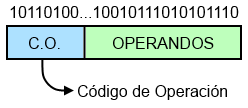
\includegraphics{res/tema1/instrucciones.png}
\end{center}

En la arquitectura de un computador Von Neumann, se tiene un modelo de computación que está basado en 3 conceptos básicos:
\begin{itemize}
\item \emph{Donde se encuentran las instrucciones}---En un computador Von Newmann, los datos y las instrucciones del programa a ejecutar están almacenadas en una \emph{única} memoria de lectura/escritura que denominamos la \emph{memoria principal}. Se denomina modelo de programa almacenado.
\item La memoria principal del computador Von Newmann es accesible por direcciones, lo que significa que cada uno de los contenidos de memoria es accesible sólo con su dirección.
\item La ejecución de las instrucciones en un computador Von Newmann es secuencial, es decir, una instrucción tras otra.
\end{itemize}

\section{Unidades principales}

TODO: AGREGAR UN DIBUJO PARECIDO AL DE LAS Diapositivas
\\\\
\begin{itemize}
\item \emph{Memoria Principal}--- Contiene las instrucciones y los datos.
\item \emph{Unidad de Entrada y Salida}--- Conecta el procesador con el resto de periféricos.
\item \emph{Unidad Central de Procesos}--- Ejecuta las instrucciones. Esta formado a su vez por 3 unidades básicas:
\begin{enumerate}
\item Unidad Aritmético Lógica--- Realiza las operaciones aritmético-lógicas de las instrucciones.
\item Unidad de Control--- Controla el computador. Da las ordenes para que los elementos del computador trabajen correctamente. Estas han de recibirse en momentos precisos dependiendo del estado del procesador, por lo que esta conectado a todos los elementos del procesador. Las instrucciones que manda son denominadas Instrucciones de Control.
\item Registros--- Elementos de almacenamiento temporal de datos de máxima velocidad de acceso.
\end{enumerate}
\end{itemize}
Conectando todos estos elementos, están los buses de datos. Conectan las diferentes partes del procesador, y la salida hacia el resto del sistema.
\\
Existen 3 tipos de buses:
\begin{itemize}
\item \emph{Bus de Direcciones}--- Direcciona la memoria principal según lo que ordene el procesador.
\item \emph{Bus de Datos}--- Vuelcan los datos entre la memoria y el procesador
\item \emph{Bus de Control}--- Manda las instrucciones (señales) del procesador para controlar otros elementos.
\end{itemize}

\section{La memoria principal}
\subsection{Direccionamiento}
Está compuesta por un conjunto de celdas del mismo numero de bits, donde se almacenan los datos y las instrucciones (Característica del modelo Von Neumann). 
A estas celdas se las denomina \emph{palabra de memoria}. 
Cada una de estas tiene asignada una dirección (0...2$^{n-1}$).
Para acceder a las palabras de memoria, basta con dar la dirección de la misma. Este sistema se denomina \emph{direccionamiento a palabra}.
\begin{center}
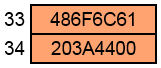
\includegraphics{res/tema1/memoriapalabra.png}
\end{center}
Existe otra forma de direccionar, que consiste en direccionar en vez de a palabra, a byte. Por ejemplo, en un sistema con una memoria de 32 bits de tamaño de palabra, una de estas contiene 4 bytes. En este sistema, cada uno de estos bytes tiene una dirección. Se denomina  \emph{direccionamiento a byte}.

\begin{center}
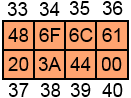
\includegraphics{res/tema1/memoriabyte.png}
\end{center}

Si el direccionamiento es a palabra, aumentamos de 1 en 1 la dirección para acceder a la siguiente palabra, y si el direccionamiento es a byte, hay que sumar el numero de bytes que puede almacenar una palabra si queremos acceder a la \textquotedblleft celda de abajo\textquotedblright
\subsection{Operación}
Para acceder a la memoria, necesitamos usar los 3 buses del procesador. La unidad de control, primero coloca en el bus de direcciones \emph{(el cual necesita n bits para poder acceder a  todas las direcciones de memoria)}, la dirección a la que quiere acceder. Entonces se manda por el bus de control la orden de acceso a memoria \emph{(memory request (MR))}, acompañada del flag del tipo de acceso que se está realizando (lectura o escritura \emph{[R/W]}).

Si se trata de un acceso de lectura, el contenido de esa dirección se recogerá entonces en el bus de datos, una vez transcurrido el tiempo de acceso que especifique el tipo de memoria.

Si se trata de un acceso de escritura, el procesador también ha de colocar en el bus de datos la información que se quiere grabar en esa dirección, y podrá quitar del bus la información una vez transcurrido el tiempo de escritura que especifique el tipo de memoria.

Es importante destacar que la escritura es destructiva, mientras que la lectura no lo es.
\subsection{Organización}
La información está habitualmente ordenada. En una zona está el código (las instrucciones), después hay una zona para los datos (estáticos o dinámicos). Al final de la memoria se sitúa la pila. Es una zona de almacenamiento que permite almacenar información y sacarla después, con un tipo de cola LIFO \emph{(Last In, First Out)}.
\\\\
La memoria tiene 3 características principales que la definen:
\begin{enumerate}
\item \emph{Capacidad}--- Se determina como el número de direcciones por el número de bits de cada dirección. También puede describirse en bytes. (Y normalmente este es el caso). Los tamaños típicos rondan los 256Mb a 16Gb en adelante.
\item \emph{Tiempo de acceso}--- Determinan los tiempos de lectura/escritura de la memoria. Normalmente están entre los 60$\sim$100 ns.
\item \emph{Tamaño de palabra}
\end{enumerate}
\section{Unidad Central de Proceso}
\subsection{Unidad Aritmético Lógica}
El ALU realiza las operaciones lógicas y aritméticas sobre cadenas de bits de longitud fija. Tiene 2 operando, y se trata de un circuito digital, por lo que tiene señales de control que le permiten seleccionar la operación. Solo puede ejecutar las ordenes para la que está diseñado. Los operandos pueden estar sobre registros o sobre memoria.
La ALU tiene un registro especial asociado, el \emph{registro de estado (RE)}. Este registro opera usando los diferentes bits del mismo como flags, y contienen información sobre la \emph{última} operación que se llevó a cabo en la ALU. Cada vez que la ALU realiza una operación, se actualiza el registro para reflejar el resultado de la misma. Los flags mas importantes son:
\begin{itemize}
\item Z \textrightarrow Resultado Cero (Se pone a valor 1 el flag si el resultado aritmetico ha sido exactamente cero)
\item OVF \textrightarrow Overflow
\item C \textrightarrow Acarreo (Carry)
\item Paridad, etc...
\end{itemize}
La salida del RE sirve para toma de decisiones, principalmente saltos condicionales.
\subsection{Modelo de ejecución del computador}
El modelo de ejecución de un computador viene definido por el lugar donde se encuentran los operandos en una instrucción aritmético-lógica. Hay 3 posibles modelos:
\begin{itemize}
\item Registro a registro (los 2 operandos en el registro)
\item Registro a memoria (un operando en registro, y otro en memoria)
\item Memoria a memoria (los 2 operandos en memoria)
\end{itemize}
Cada modelo de ejecución contiene al anterior. P.E; en el modelo de memoria a memoria pueden provenir también de registros.
\subsection{Registros}
Son elementos de almacenamiento temporal, ubicados en el procesador. Son extremadamente rápidos. Hay de 3 tipos:
\begin{itemize}
\item de propósito general
\subitem Banco de registros
\item de propósito especifico
\subitem PC \textrightarrow Contador de Programa (Program Counter)
\subitem SR \textrightarrow Registro de Estado (State Regisry)
\subitem SP \textrightarrow Puntero de Pila (Stack Pointer)
\item transparentes
\subitem IR \textrightarrow Registro de Instrucción (Instruction Register)
\subitem AR \textrightarrow Registro de Direcciones (Adress Register)
\subitem IR \textrightarrow Registro de Datos (Data Register)
\end{itemize}
Los registros de propósito general se usan explícitamente en el juego de instrucciones del computador. Pueden ser usados por cualquier instrucción que lleve a cabo operaciones sobre datos. Se suelen agrupar en bancos de registros, y tienen un tamaño igual al de la palabra.

Los registros de propósito especifico tienen su uso restringido a determinadas instrucciones, y suelen usarlo de forma implícita.

Los registros transparentes son los que usa internamente el procesador, y no se especifican en las instrucciones. No son accesibles fuera de la unidad central de proceso.
\end{document}